TODO Revoir l'ordre

\section{Notion de translation --- Vecteur associé}
\subsection{Définitions}

\begin{definition}
  Soient $A$ et $B$ deux points du plan.
  \begin{itemize}
    \item On appelle \emph{translation qui transforme $A$ en $B$} la transformation qui a tout point $C$ du plan associe l'unique point $D$ tel que $[AD]$ et $[BC]$ ont même milieu.
    \item À cette translation, on associe le \emph{vecteur $\vecteur{AB}$}, qui symbolise le déplacement de $A$ vers $B$ (ou de $C$ vers $D$).
    \item Le point $A$ est appelé \emph{l'origine} du vecteur $\vecteur{AB}$, et le point $B$ son \emph{extrémité}.
    \item On dit que $B$ est \emph{l'image} de $A$ par la translation de vecteur $\vecteur{AB}$.
  \end{itemize}
\end{definition}

\begin{remarque}
  Si les points $A$ et $B$ sont confondus, tout point $C$ est également confondu avec son image par la translation de vecteur $\vecteur{AB}$. On dit aussi que tout point du plan est \emph{invariant} par la translation de vecteur $\vecteur{AB}$.

  Le vecteur $\vecteur{AA}$ est appelé \emph{vecteur nul}, et on note $\vecteur{AA}=\vecteur{0}$.
\end{remarque}

\begin{propriete}[Propriétés d'une translation]
  Soient $A$ et $B$ deux points du plan, $M$, $N$ et $O$ trois points ayant pour image respective $M'$, $N'$ et $O'$ par la translation de vecteur $\vecteur{AB}$. Alors :
  \begin{itemize}
    \item Si $M$, $N$, et $O$ sont alignés, alors $M'$, $N'$ et $O'$ sont alignés.
    \item L'image du segment $[MN]$ est le segment $[M'N']$, de même longueur.
    \item Si $O$ est le milieu de $[MN]$, alors $O'$ est le milieu de $[M'N']$.
  \end{itemize}

  On dit que la translation conserve les angles et les distances :

  \begin{itemize}
    \item L'image d'une droite par une translation est une droite parallèle.
    \item L'image d'un cercle par une translation est un cercle de même rayon.
  \end{itemize}
\end{propriete}

\subsection{Égalité de vecteurs}

\begin{definition}
  Deux vecteurs sont dit $\emph{égaux}$ s'ils sont associés à une même translation.
\end{definition}

\begin{propriete}
  Soient $A$, $B$, $C$ et $D$ quatre points distincts du plan. Les propriétés suivantes sont équivalentes.
  \begin{itemize}[$\bullet$]
    \item $\vecteur{AB}=\vecteur{CD}$.
    \item $D$ est l'image de $C$ par la translation qui transforme $A$ en $B$.
    \item $[AD]$ et $[BC]$ ont le même milieu.
    \item $ABDC$ est un parallélogramme (éventuellement aplati).
  \end{itemize}
\end{propriete}

\begin{definition}
  Pour désigner l'unique vecteur associé à la translation qui transforme $A$ en $B$ et $C$ en $D$, on peut utiliser une lettre unique en écrivant $\vecteur{AB}=\vecteur{CD}=\vecteur{u}$.

  On dit alors que les vecteurs $\vecteur{AB}$ et $\vecteur{BC}$ sont les \emph{représentants} du vecteur $\vecteur{u}$.
\end{definition}

\begin{remarque}
  Une vecteur admet une infinité de représentants.
\end{remarque}

\begin{propriete}
  Un vecteur non nul $\vecteur{AB}$ est déterminé par 
  \begin{itemize}
    \item sa direction (celle de la droite $(AB)$) ;
    \item son sens (de $A$ vers $B$) ;
    \item sa longueur, $AB$, appelée \emph{norme} du vecteur, et notée $\norme{\vecteur{AB}}$.
  \end{itemize}
\end{propriete}

\begin{corollaire}
  Deux vecteurs non nuls sont égaux si et seulement s'ils ont même direction, même sens et même longueur.
\end{corollaire}

\begin{remarque}
  Le vecteur nul n'a ni direction, ni sens.
\end{remarque}

\begin{propriete}[Caractérisation du milieu]
  Le point $I$ est le milieu du segment $[AB]$ si et seulement si les vecteurs $\vecteur{AI}$ et $\vecteur{IB}$ sont égaux.
\end{propriete}

\section{Somme de deux vecteurs}

\begin{activite}
\tikzstyle{point}=[draw, shape=circle, fill=black, inner sep=0pt, minimum size=5pt]
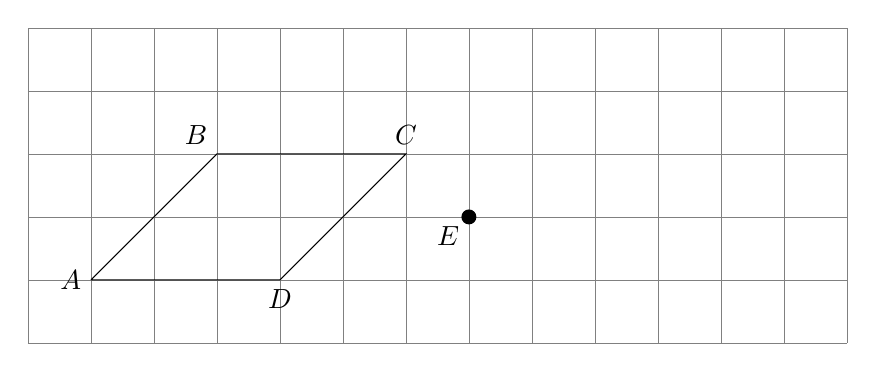
\begin{tikzpicture}[scale=0.8]
  \draw[very thin,color=gray,step=1] (0,0) grid (13,5);
  \draw (1,1) -- (3,3) -- (6,3) -- (4,1) -- (1, 1);
  \node[left] at (1,1) {$A$};
  \node[above left] at (3,3) {$B$};
  \node[above] at (6,3) {$C$};
  \node[below] at (4,1) {$D$};
  \node[below left] at (7,2) {$E$};
  \node[point] at (7,2) {};
\end{tikzpicture}

\begin{enumerate}[(a)]
  \item Placer le point $F$ tel que $\vecteur{EF}=\vecteur{AB}$.
  \item Placer le point $G$ tel que $\vecteur{FG}=\vecteur{BC}$.
  \item Placer le point $H$ tel que $\vecteur{EH}=\vecteur{AC}$.
  \item Que remarquez-vous ? Comment traduire cela par une égalité de vecteurs ?
\end{enumerate}
\end{activite}

\begin{propriete}[Relation de Chasles]
  Pour tous points $A$, $B$, $C$ du plan, on a :

\[\vecteur{AB}+\vecteur{BC}=\vecteur{AC}\]
\end{propriete}

\begin{definition}
  Soient $\vecteur{u}$ et $\vecteur{v}$ deux vecteurs. On appelle
  \emph{somme} des vecteurs $\vecteur{u}$ et $\vecteur{v}$, le vecteur
  $\vecteur{w}$ associé à la transformation résultant de l'enchaînement des
    translations de vecteur $\vecteur{u}$ et $\vecteur{v}$.
  \end{definition}

\section{Produit d'un vecteur par un réel}

\begin{definition}
  Soint $\vecteur{u}$ un vecteur non nul, et $k$ un réel non nul. On appelle \emph{produit de $k$ par $\vecteur{u}$} le vecteur noté $k\vecteur{u}$ :
  \begin{itemize}
    \item de même direction que $\vecteur{u}$ ;
    \item de même sens si $k>0$, et de sens opposé si $k<0$ ;
    \item de norme égale à $\systeme{k\norme{\vecteur{u}}\text{ si $k>0$}}{-k\norme{\vecteur{u}}\text{ si $k<0$}}$.
  \end{itemize}
\end{definition}

\begin{definition}[Cas particuliers]
  Soit $\vecteur{u}$ un vecteur non nul, et $k$ un nombre réel non nul.
  \begin{itemize}
    \item $0\vecteur{u}$ est égal au vecteur nul $\vecteur{0}$ ;
    \item $k\vecteur{0}$ est égal au vecteur nul $\vecteur{0}$.
  \end{itemize}
\end{definition}

\begin{propriete}
  Soit $\vecteur{u}$ un vecteur nul. Le vecteur $-\vecteur{u}$ est le vecteur de même direction, de même norme, et de sens opposé à $\vecteur{u}$.
\end{propriete}

\begin{propriete}
  Pour tous points $A$ et $B$, $-\vecteur{AB}=\vecteur{BA}$.
\end{propriete}

\begin{definition}[Différence de deux vecteurs]
  Étant donnés deux vecteurs $\vecteur{u}$ et $\vecteur v$, on appelle
  \emph{différence} de $\vecteur u$ et $\vecteur v$, le vecteur $\vecteur w$, noté \emph{$\vecteur{w}=\vecteur{u}-\vecteur{v}$} tel que :

  \[\vecteur u-\vecteur v=\vecteur u + (-\vecteur v)\]
\end{definition}

\begin{definition}
  Deux vecteurs $\vecteur{u}$ et $\vecteur{v}$ sont \emph{colinéaires} si l'un des deux est le vecteur nul, ou s'il existe un réel $k$ tel que $\vecteur{u}=k\vecteur{v}$.
\end{definition}

\begin{propriete}
  Soient $A$, $B$, $C$ et $D$ quatre points du plan.
  \begin{itemize}
    \item Les droites $(AB)$ et $(CD)$ sont parallèles si et seulement si $\vecteur{AB}$ et $\vecteur{CD}$ sont colinéaires.
    \item Les points $A$, $B$ et $C$ sont alignés si et seulement si les vecteur $\vecteur{AB}$ et $\vecteur{CD}$ sont colinéaires.
  \end{itemize}
\end{propriete}

\section{Coordonnées de vecteurs}

TODO Se placer dans un repère de points

\begin{definition}
  Le plan est muni d'un repère $(O, \vecteur\imath,
  \vecteur\jmath)$. Pour tout vecteur $\vecteur u$ du plan, il existe un unique
  couple $(x,y)$ de réels tels que $\vecteur
  u=x\vecteur\imath+y\vecteur\jmath$.

Ce couple est appelé \emph{coordonnées de $\vecteur{u}$}, et on note
$\vecteur{u}(x;y)$ ou
$\vecteur{u}\coord{x}{y}$.
\end{definition}

\begin{definition}[Coordonnées d'un point]
  TODO
\end{definition}

\begin{propriete}
  Soient $A(x_A,y_A)$ et $B(x_B,y_B)$ deux points du plan. Alors les coordonnées du vecteur $\vecteur{AB}$ sont $(x_B-x_A;y_B-y_A)$.
\end{propriete}

\begin{propriete} Soient deux vecteurs $\vecteur u\coord{x}{y}$ et $\vecteur v\coord{x'}{y'}$.
  \begin{enumerate}
  \item Les vecteurs $\vecteur u$ et $\vecteur v$ sont égaux si et seulement si $x=x'$ et $y=y'$.
  \item Les coordonnées du vecteur $\vecteur u+\vecteur v$ sont $\coord{x+x'}{y+y'}$.
  \item Soit un réel $k$. Les coordonnées du vecteur $k\vecteur u$ sont $\coord{kx}{ky}$.
\item $\vecteur u$ et $\vecteur v$ sont colinéaires si et seulement si il existe un réel $k$ tel que $\left\{\begin{array}{l}x'=kx\\y'=ky\end{array}\right.$.
\end{enumerate}
\end{propriete}

\begin{propriete}[Condition de colinéarité]
  TODO
\end{propriete}
